\documentclass[12pt,oneside]{article}
\usepackage{thesis} % use thesis style file
\begin{document}
%===============================================================================
% TITLE PAGE / ABSTRACT / ACKNOWLEDGEMENTS
%===============================================================================
% \frontmatter % this is the stuff that comes before the real text:
% %Here goes the title page:
\pagestyle{empty}
\begin{titlepage}
\begin{center}
\rule{5.75in}{1pt} \\
\vspace*{-0.125in}
{\large \doublespacing Wesleyan University} \hfill {\large \doublespacing The Honors College}
\rule[0.2in]{5.75in}{1pt} \\
\vspace*{0.8in}

% title
{\LARGE \singlespacing \bf 
  Using Vertical Structure to Infer \\
  the Dynamical Mass Hidden in \\
  the AU Mic Debris Disk
  } \\
\vspace*{0.05in}
\vspace*{0.10in}

{\large \vspace*{0.20in}  \singlespacing by \vspace*{.2in}
\\Cail Daley \\ Class of 2018\\}
\vspace*{0.25in}
\vspace*{0.8in}
{\large \singlespacing A thesis submitted to the\\ faculty of Wesleyan University\\ in partial fulfillment of the requirements for the \\ Degree of Bachelor of Arts\\ with Departmental Honors in Astronomy\\ \vspace*{-0.15in} }
\vspace*{.25in}
\rule{5.75in}{1pt} \\
\vspace*{-0.125in}
{\large \doublespacing Middletown, Connecticut \hfill April, 2018}
\rule[0.2in]{5.75in}{1pt} 
\end{center}
\end{titlepage}

% \pagestyle{empty}
% %\pagestyle{plain}

\mbox{}
\vspace{.75in}
\hrule

\vspace{2in}


%\begin{minipage}[c]{4in}
\begin{centering}
	\hspace{.25in} 
	\parbox{5in}{
		\noindent 
		\textit{We are just an advanced breed of monkeys on a minor planet of a very average star. But we can understand the Universe. That makes us something very special.}
		\vspace{3pt}

		\begin{flushright}
			{\sc {--Stephen Hawking}}\\
		%	{\textit{The Hitchhiker's Guide to the Galaxy}}
		\end{flushright}
	}
\end{centering}
\vspace{2.25in}
\hrule
\vfill



%\flushleft















\textwidth 5.750in \textheight=8.50in \headheight 0.0625in \topmargin 0.0in % book strict

% \chapter{Acknowledgements}

I would like to thank Meredith Hughes for being an amazing mentor through the process of teaching me to do advanced research, all the way from the crash course in radio astronomy at the beginning of my Junior year through this thesis. I'm blessed to have worked with such a dedicated advisor who cares so much about the learning process for each and every student. Going to Hawaii to observe at the SMA and Seattle for AAS were unforgettable experiences that not many undergraduates have, but those are really just cherries on top of the incredible sundae of knowledge, experience, and wisdom that you've passed on to me. 

Thanks to Seth Redfield for selling me on the astronomy program here at Wesleyan and getting me involved with the 24$''$ observing program. I may never live down getting flung from my chair as the monkey in an angular momentum demonstration he put me up to, but at least I'm better at ultimate frisbee. 

Thanks to Kevin Flaherty, for helping me out with everything from cluster computing to statistical tests, and to Roy Kilgard, for the endless patience in helping me with computer issues and always being fun to stop by and talk to. Thanks to Angelo Ricarte for writing the foundation of the modeling code that I used in this thesis. 

To Mom and Dad, thanks for giving me multiplication problems before bed to help me fall asleep, even if you didn't always know the correct answer. I wouldn't be who I am today without your love and guidance. Mira, you're the best sister a little bro could ask for. 

To the basement crew, thanks for endless entertainment in times of drastic procrastination, playing darts, and letting me fly the baby drone around the library when that was our workspace without going crazy (RIP baby drone. Both a sorry and a damn you to the Fisk Telescope for breaking the last propellor). 

\titlespacing*{\chapter}{0pt}{*2}{*3}

%===============================================================================
% TABLE OF CONTENTS
%===============================================================================
% \tableofcontents % \pagestyle{empty}
%\listoffigures
%\listoftables \pagestyle{empty}
%===============================================================================
% sectionS
%===============================================================================
% \mainmatter 
% \chapter{Observations}
\label{chap:obs}


\section{Introduction}
\label{section: introduction}

Planets form during a relatively short and early stage in the lifetime of stellar systems,  when the host star is still encircled by a `protoplanetary' disk rich in gas. 
In fact, planets and smaller planetesimals derive their substance from these reservoirs of gas and dust.
As such, planet formation (as well as processes including accretion, photoevaporation, and winds) causes first-generation protoplanetary material to dissipate over time \citep{williams&cieza11,ercolano&pascucci17}.
The first-generation material is replaced by second-generation `debris,' produced by a collisional grinding of larger (Pluto-sized) planetesimals into small dust grains in a process know as a collisional cascade \citep{wyatt2008}. 
The resulting debris disks, optically thin and significantly less luminous than their protoplanetary counterparts, are found around at least 25\% of Solar-type stars and are likely to be as common as the high observed frequency of exoplanetary systems exoplanetary systems with which they are thought to be associated \citep{montesinos16}.

Analysis of their morphological and emissive properties sheds light on the final stages of planetary system evolution and can reveal the presence of planets hidden within.
Planets can imprint features such as rings/gaps, clumps, or other asymmetries on their parent disks, although it is rarely straightforward to infer the properties of planets directly from the disk morphology (A. M. Hughes et al., in prep).
In gas-poor systems, the vertical structure of a debris disk can serve as a probe of the total mass of large bodies stirring the collisional cascade.
The presence of massive bodies increases the inclination dispersion  of the constituent dust particles and thus the scale height $H$ of the observed dust distribution.

The dynamical excitation of a disk an therefore be measured from its aspect ratio $H/r$, which in turn allows inferences about the presence and size of the bodies responsible for the dynamical stirring.
Such work has been undertaken by several authors using visible and infrared observations \citep{artymowicz97,thebault&augereau07,quillen07}.
However, \cite{thebault09} demonstrate that radiation pressure from the host star should excite the smallest dust grains, imparting `natural' scale height to the disk even in the absence of large bodies dynamically stirring the disk. 
Thus longer-wavelength ($\lambda \geq \SI{50}{\mu m}$) observations are required to measure disk scale height as determined by dynamical stirring alone, since the grains dominating the emission are large enough to be impervious to the effects of radiation pressure.

The M3IVe star AU Mic presents a particularly favorable target for such observations due to its proximity (\SI{9.91}{pc}; \citealp{vanleeuwen07}) and edge-on inclination. 
The first M star detected to have a far-infrared excess, AU Mic hosts one of the best-studied debris disks. 
As a member of the $\beta$ Pic Moving Group, it is thought to be relatively young: $\SI{23 \pm 2}{Myr}$ \citep{binks&jeffries14,mamajek&bell14,malo14}. 
The disk around AU Mic was first resolved by \cite{kalas04} in scattered light, and a host of observations spanning the optical to the submillimeter have followed \citep{augereau&beust06,macgregor13,matthews15,schneider14,wang15}. 
Notably, the debris around AU Mic exhibits a so-far-unique time variability at scattered light wavelengths.
\cite{boccaletti15} identify five features--local intensity maxima offset from the disk midplane--on the SE side of the disk. 
These features are quickly moving away from the star along the disk midplane at projected velocities that are not consistent with Keplerian rotation; in fact, the outermost two features appear to be unbound to the star. Both dust emission from a localized source such as a planet \citep{boccaletti15,sezestre17} and collisional dust avalanches \citep{chiang&fung17} have been proposed to explain these features.\footnote{I've really no idea which of AU Mic's observed characteristics I should mention here.. I figured that the Boccaletti paper is one of the most interesting to the average reader, but I'm sure I missed some other important bits.}

Here we present new \SI{0.4}{''} Atacama Large Millimeter/submillimeter Array \newline (ALMA) \SI{1.3}{mm} observations of the AU Mic debris disk. 
These observations represent a factor of $\sim 2$ improvement in both spatial resolution and rms noise relative to \cite{macgregor13}, and are the first to resolve a debris disk in both the radial and vertical directions at millimeter wavelengths. 
In Section \ref{section: observations} we present the new observations and describe the data reduction.  
Section \ref{section: results} quotes the basic observational results and compares the millimeter morphology of the disk with the morphology at shorter wavelengths.  
In Section \ref{section: analysis} we conduct a parametric exploration of a 2-dimensional disk model in order to investigate the degeneracy between vertical structure, radial structure, and viewing geometry.
In Section \ref{section: discussion} we discuss our results, particularly the constraints on the dynamical excitation of the disk imposed by our measurement of the scale height, and compare them to previous observations.
“The results of our measurement of scale height and its implications for the total disk mass are summarized in Section 6.” 



\section{Observations}
\label{section: observations}
AU Mic was observed  with ALMA on three dates: 26 March 2014, 18 August 2014, and 24 June 2015 (see Table \ref{tab:observations}). 
All observations employed ALMA's 12m antennas and Band 7 receivers, including four independently tunable spectral windows. 
One spectral window was centered around the CO $J = (2-1)$ transition at a rest frequency of 230.538001 GHz, with a total bandwidth of 1.875 GHz and a channel spacing of \SI{0.6}{km/s}.
The remaining three spectral windows were configured to detect continuum emission with central frequencies of 228.5, 213.5, and 216.0 GHz, total bandwidths of 2 GHz, and channel spacings of \SI{21.7}{km/s}.

% The long-baseline August data were supplemented with a second night of higher-quality observations (as indicated by the relative pwv levels) in June 2015.
% The short-baseline March observation provides information about AU Mic's disk on large spatial scales; in contrast, the subsequent long-baseline August observation was intended to trace the small-scale structure of the disk. 

\begin{table}	
  \centering
	\caption{Observation Information}
  \label{tab:observations}
  \begin{tabular}{lrrrr}
    \toprule
                    & 26 March 2014 & 18 August 2014 & 24 June 2015 \\
    \cmidrule(lr){2-4}
    Antennas:             & 32         & 35            & 37 \\
    Baseline length (m):  & 14--437    & 20--1268      & 30--1431 \\
    On-source time (min): & 35         & 35            & 33 \\
    Flux calibrator:      & Titan      & J2056-472     & Titan \\
    Bandpass calibrator:  & J1924-2914 & J2056-4714    & J1924-2914 \\
    Phase calibrator:     & J2101-2933 & J2101-2933    & J2056-3208 \\
    Gain Calibrator:      &            & J2057-3734    & J2101-2933 \\
    pwv (\si{mm}):        & 0.6        & 1.6           & 0.7 \\
    \bottomrule
  \end{tabular}
\end{table}

Calibration, reduction, and imaging were carried out using the \texttt{CASA} and \texttt{MIRIAD} software packages. Standard ALMA reduction scripts were applied to the datasets: phase calibration was accomplished via water vapor radiometry tables, and system temperature calibrations were performed to account for variations in instrument and weather conditions. 
Flux and bandpass calibrations were subsequently applied.

During the last segment of the June observation (04:23:38-04:29:58 UT), the host star flared. 
To determine the flux of the flare as a function of time, we binned the data into one-minute intervals using the \texttt{CASA} task \texttt{split} and fit a point source in each bin to baselines between \SI{100}{\kilo \lambda} and \SI{1400}{\kilo \lambda} with \texttt{uvmodelfit}. 
The resulting flare fits can be found in Table \ref{tab:flare fluxes}. 
We exclude from our analysis the seven minutes during which the flare occurred, as it proved difficult to separate the stellar emission from the disk emission while it was changing so rapidly.

\begin{table}	
  \centering
	\caption{Central point source flux before and during the June flare}
  \label{tab:flare fluxes}
  \begin{tabular}{lr}
    \toprule
    Time (UTC) & Point-source Flux ($\mu$Jy) \\
    \midrule
    03:45:0--04:20:0 (no flare) & ($4.1 \pm 0.2)  \times 10^2$\\
  	4:23:38--4:24:00 & $(9.2 \pm 1.7) \times 10^2$ \\
  	4:24:00--4:25:00 & $(1.146 \pm 0.010) \times 10^4$ \\
  	4:25:00--4:26:00 & $(3.59 \pm 0.10) \times 10^3$ \\
  	4:26:00--4:27:00 & $(1.58 \pm 0.10) \times 10^3$ \\
  	4:27:00--4:28:00 & $(4.50 \pm 1.0) \times 10^2$ \\
  	4:28:00--4:29:00 & $(4.60 \pm 1.0) \times 10^2$ \\
  	4:29:00--4:29:58 & $(5.20 \pm 1.0) \times 10^2$\\
    \bottomrule
  \end{tabular}
\end{table}


Since AU Mic is a high proper motion system, its equatorial coordinates changed rapidly over the 1.5 years between observations.  
We were able to obtain a more precise alignment of the data sets using the bright chromospheric emission from the central star than from the measured proper motion
We fit an image-domain elliptical gaussian to a small region around the star on each date with the task \texttt{imfit}, and used the centroid of the Gaussian fit to define the star position.
We note that for the June data, the exclusion of the flare changed the centroid of the Gaussian fit by \SI{.076 \pm 0.002}{''}, i.e. $\sim 2$ pixels; this could be explained if the flare were not symmetric with respect to the star.
Finally, each dataset was phase shifted using the task \texttt{fixvis} so that the pointing center of the data was the same as the fitted star position.

Imaging was performed using standard Fourier inversion methods as implemented in the \texttt{CASA} task \texttt{tclean}. 
Two weighting schemes were used: (i) natural weighting with no taper to trace the small-scale disk structure and (ii) natural weighting with a \SI{200}{k\lambda} Gaussian taper applied to long baselines to bring out the disk emission on larger spatial scales. 
In scheme (i) the rms noise ($\sigma$) was \SI{14.8}{\mu Jy / beam} and the restoring beam was $\SI{0.52}{''} \times \SI{0.39}{''}$ with a position angle (PA) of \ang{77.9}. 
In scheme (ii), the corresponding values are \SI{19.2}{\mu Jy / beam}, $\SI{0.87}{''} \times \SI{0.71}{''}$, and \ang{80.8}
Because the \texttt{CASA} task \texttt{tclean} preserves pointing center offsets when converting several visibility datasets into an image, it was necessary to combine the data into a single file (with a common pointing center) before clearning before cleaning in order to account for the offset in phase center between datasets. 
This was done using the task \texttt{concat}, which combines datasets with pointing centers aligned so long as their pointing centers do not differ by a value greater than the parameter \texttt{dirtol}).


\section{Results}
\label{section: results}

Figure \ref{fig: aumic_imaged} shows the combined dust continuum emission from all three observations at \SI{1.3}{mm}; chromospheric emission from the M star is visible as a point source at the center of the image \citep{cranmer13}. 
We report the integrated flux of the $3 \sigma$ regions of the source emission to be \SI{4.97 \pm 0.08}{\milli Jy}; considering that we derive an average stellar flux of \textbf{not here yet} (see Section \ref{section: analysis}), we estimate the total disk flux to be \textbf{not here yet}.
The ansa to the NW exhibits a maximum flux density of \SI{330 \pm 20}{\mu Jy/beam} at a separation of \SI{24.8}{au} and PA of \ang{128.30}, while the ansa to the SE exhibits a maximum flux density of \SI{340 \pm 20}{\mu Jy} at a separation of \SI{29.0}{au} and PA of \ang{128.69}, yielding a disk peak signal-to-noise of $\sim23$. 
The ansae peak flux densities differ by roughly the rms noise, indicating that there is no significant difference in brightness between the two limbs of the disk.
Indeed, the apparent flux asymmetry in these data is in the opposite direction of the apparent flux asymmetry in \cite{macgregor13}, providing further circumstantial evidence that there is no significant flux asymmetry at millimeter wavelengths. 
Additionally, the discrepancies in PA between the two peaks do not attain significance and so we are not able to confirm the scattered light PA offset observed by \cite{boccaletti15}. 

The radial structure of AU Mic's disk is traced in Figure \ref{fig: boccaletti}. 
At each radial location along the disk major axis, a one-dimensional Gaussian was fit to the surface brightness profile perpendicular to the major axis.
In descending order, the three panes correspond to the amplitude, centroid, and beam-subtracted FWHM of the Gaussian fits; broadening effects of the synthesized beam in the vertical direction have been removed by subtracting in quadrature the Gaussian beam FWHM from the Gaussian fit FWHM.
In more physical terms, the three panes show the disk `spine' intensity, the spine's elevation from the disk midplane, and the disk FWHM.
We are not able to detect the intensity variations or excursions of the disk spine from the midplane that characterize the fast-moving features observed by \cite{boccaletti15}.
This is not entirely surprising, as \cite{sezestre17} and \cite{chiang&fung17} suggest the clouds to be composed of sub-micron-sized grains, which do not emit efficiently at wavelengths to which our observations are sensitive.

The disk is resolved across $\sim13$ beams along the major axis, and cursory image-domain analysis indicates the disk is marginally resolved perpendicular to the major axis as well (Figure \ref{fig: boccaletti}, bottom pane).
$3\sigma$ emission extends to a distance of $\sim \SI{43.2}{au}$ on the NW side, and $\sim \SI{45.9}{au}$ on the SE side, as seen in the top pane of Figure \ref{fig: boccaletti}. 
We note the presence of local intensity maxima, symmetric about the star at a distance of $\sim \SI{1}{au}$; it is unclear if these are real features of the disk or are artifacts of the rms noise or cleaning process. 
We examine the significance of these features more carefully in Section \ref{section: analysis} below.

\begin{figure}
  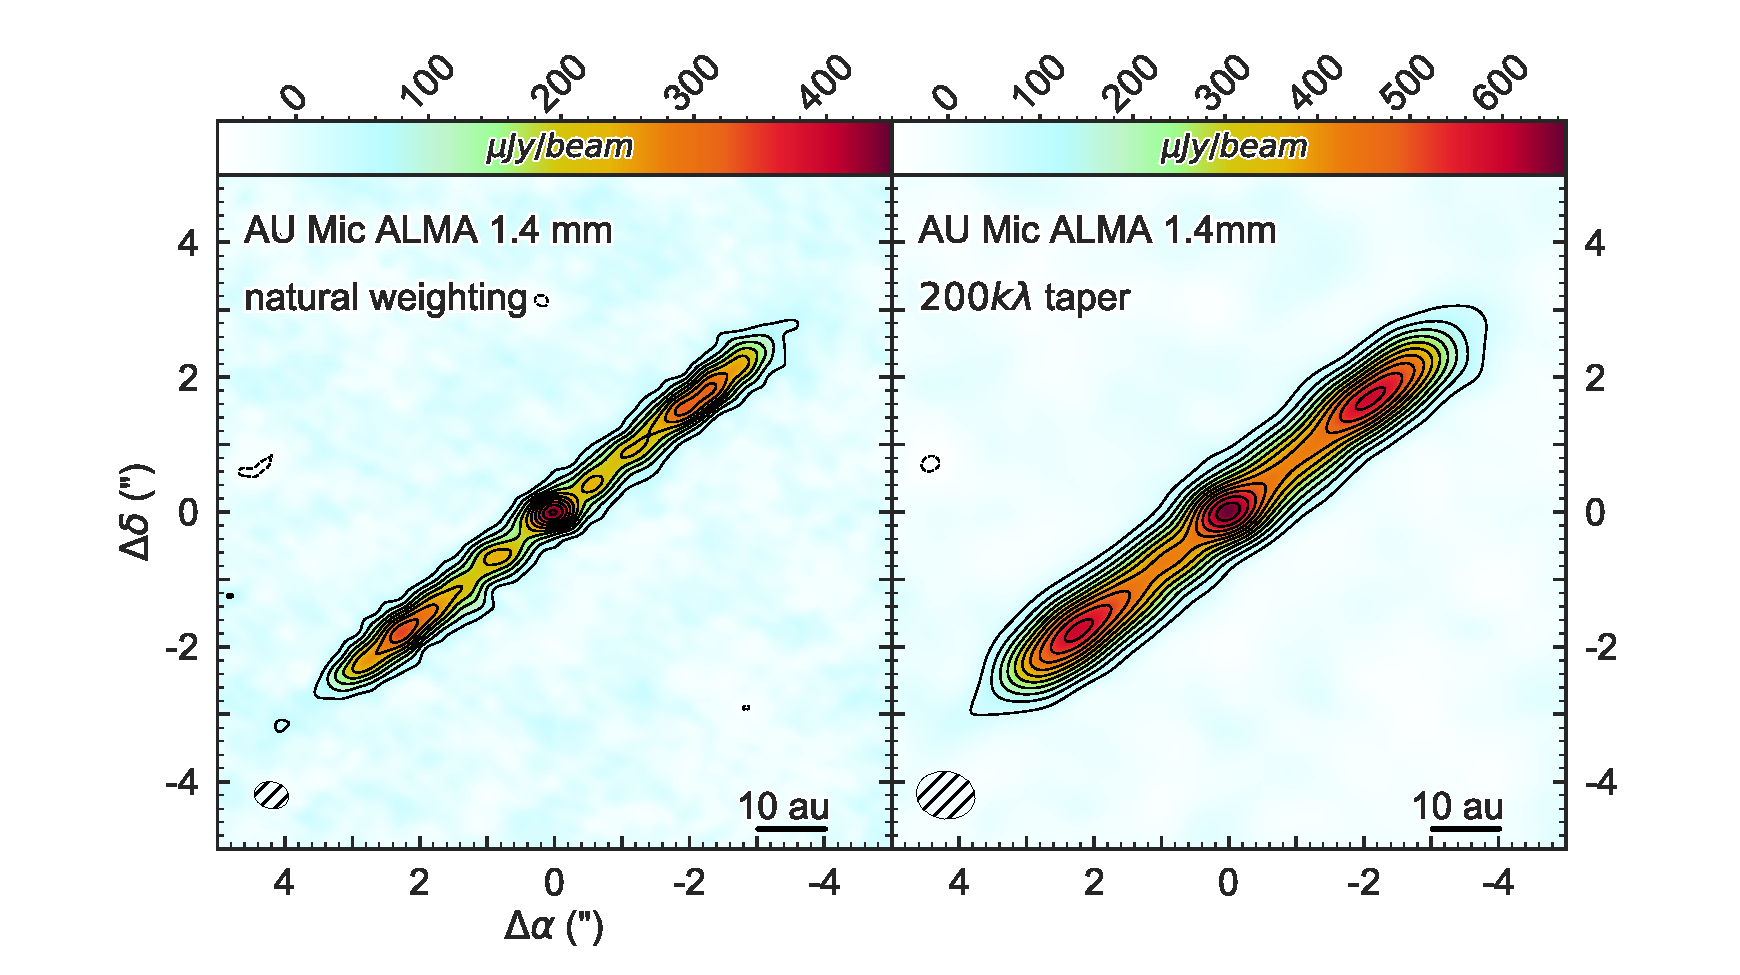
\includegraphics[width=\linewidth]{figures/aumic_imaged}
  \caption{The AU Mic system imaged by ALMA at a wavelength of \SI{1.4}{mm}, using natural weighting with and without a Gaussian taper on the long baselines. 
  For the untapered weighting, the rms noise is \SI{14.8}{\mu Jy / beam} and the restoring beam has dimensions $\SI{0.52}{''} \times \SI{0.39}{''}$ with a PA of \ang{77.9}.
  The corresponding values for the tapered weighting are \SI{19.2}{\mu Jy / beam}, $\SI{0.87}{''} \times \SI{0.71}{''}$, and \ang{80.8}. 
  The hatched ellipse in the bottom left of each pane designates the size and shape of the restoring beam.
  }
  \label{fig: aumic_imaged}
\end{figure}


\begin{figure}
  \centering
  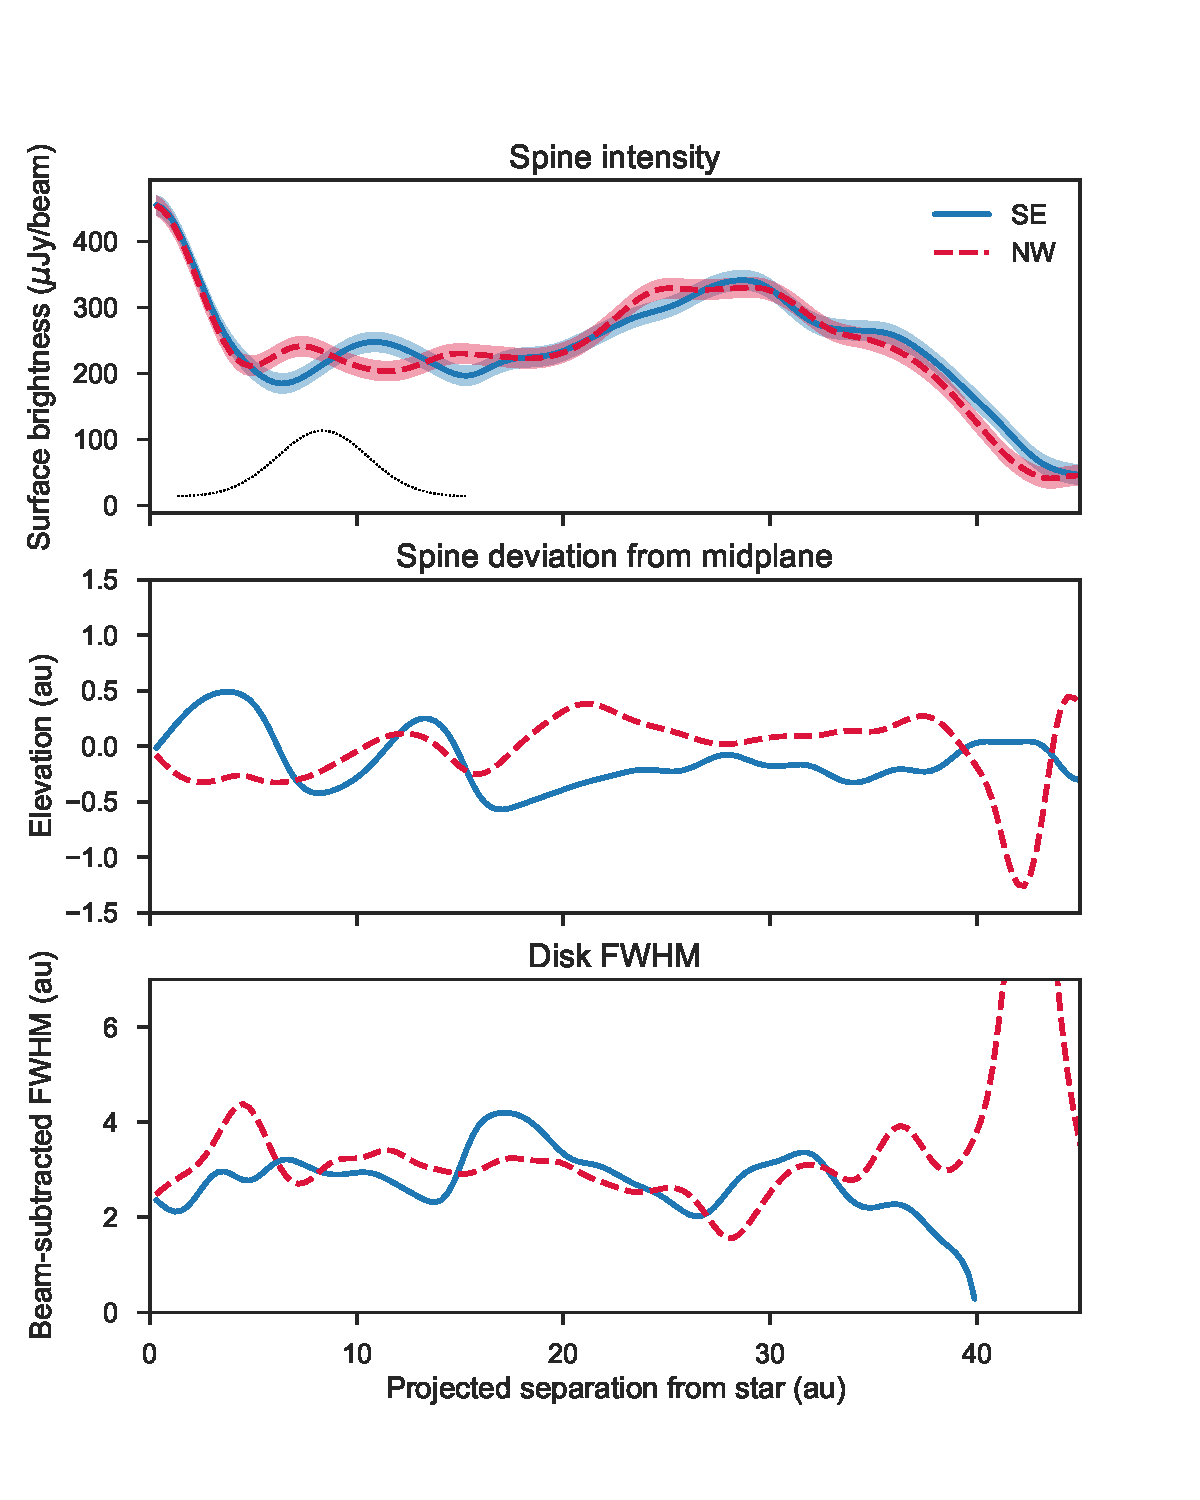
\includegraphics[width=.75\linewidth]{figures/boccaletti_plots}
  \caption{
  Image-domain analysis of the AU Mic debris disk radial and vertical structure. 
  From top to bottom, the three panes show as a function of projected separation from the star i) the disk spine surface brightness, ii) the disk spine deviation from the midplane, iii) the disk FWHM. 
  The Gaussian traced by the dotted line in the upper pane shows the width of the  synthesized beam in the radial direction.
  The fact that the image-domain vertical height of the disk is in excess of the beam contribution implies that our data spatially resolve the vertical structure of the disk.} 
  \label{fig: boccaletti}
\end{figure}



\section{Analysis}
\label{section: analysis}
Previous studies of the scale height of debris disks have demonstrated a degeneracy between vertical structure, radial structure, and viewing geometry \citep[e.g.][]{milli14}.  
The modeling approach we adopt is designed to use appropriate ray tracing along with MCMC methods to investigate the degree to which these known degeneracies impact our ability to measure the vertical structure of the disk.  
We use the parametric structure and ray tracing disk code described in \cite{flaherty15}, itself an adaptation of earlier work by \cite{rosenfeld13}.
Synthetic sky-projected images are generated from an assumed temperature and density structure and are subsequently Fourier transformed to create model visibilities that can be directly compared to the interferometric data.

We assume the disk to be azimuthally symmetric and vertically isothermal. 
The disk vertical density structure at a given radius $r$ is assumed to be Gaussian with a standard deviation defined by the scale height $H=hr$, where the coefficient $h$ is the disk aspect ratio.
The dust grains are assumed to be in blackbody equilibrium with the central star, so the dust temperature a distance $d$ from the host star is given by
\begin{align}
  T_{dust} &= \left( \frac{L_{\star}}{16 \pi d^2 \sigma} \right)^{1/4}
\end{align}
where $L_{\star}$ is the bolometric luminosity of the star and $\sigma$ is the Stefan-Boltzmann constant. We assume\footnote{There are an awful lot of `assume's in this section.. Are there other phrases/verbs I can use to vary the language a little bit?} that the radial surface density takes the form of a power law: 
\begin{align}
\Sigma(r) &= \begin{cases}
\Sigma_0 \, r^{p} \; \; \; \; & r_{in} \leq r \leq r_{out} \\
0 \; \; \; \; &\mbox{otherwise} 
\end{cases}
\end{align}
where $p$ is the power law exponent, and $r_{in}$ and $r_{out}$ are the disk inner and outer radius. 
$\Sigma_0$ normalizes the surface density structure for a given total dust mass $M$:
\begin{align}
\Sigma_c &= \frac{M \left(p + 2 \right)}{2 \pi \left[ r_{out}^{(p+2)} - r_{in}^{(p+2)} \right]}.
\end{align}

Once the temperature and density grids are defined, a sky-brightness model image is created for a given set of observational parameters using a ray tracing algorithm. We assume a stellar luminosity of \SI{0.09}{\Lsun} and a distance to the star of \SI{9.91}{pc}; the observed \SI{1.3}{mm} stellar flux $F_\star$ is left as a free parameter for each observation date \citep{plavchan09,vanleeuwen07}.
The ray tracing assumes an observed inclination $i$ and PA, both of which are free parameters.
The dust opacity is set to \SI{2.3}{\cm^2 / \gram}, placing the model disk in the optically thin regime for the range of dust masses explored.\footnote{This is correct, right? I'm pretty sure we decided that the problems we were having with the skinny disk run were caused gridding rather than optical depth effects.} 
The spatial resolution of the resulting model sky image is set to \SI{0.3}{au} per pixel, i.e. \SI{10}{\percent} of the spatial scale sampled by the longest baseline in the data. 
The model image is subsequently sampled at the same spatial frequencies as the ALMA data and Fourier transformed into the visibility domain with the \texttt{MIRIAD} task \texttt{uvmodel}. 
This allows the model to be compared directly to the interferometric data, for which the uncertainties are better understood.
A $\chi^2$ metric is used to asses the quality of the fit.

We explore the parameter space of the model using a Markov Chain Monte Carlo (MCMC) routine. 
Specifically, we use the affine-invariant formulation described by \cite{goodmanweare10} and implemented in Python as \texttt{emcee} \citep{foreman-mackey13}.  
MCMC methods sample parameter space such that the resulting sample distribution is proportional to the probability distribution, allowing the posterior probability function of each parameter to be estimated. 
As such, the process not only identifies regions of high probability in parameter space, but uncertainties and degeneracies between parameters can be determined by examining the correlations between the posteriors of each parameter.

\begin{table}
  \caption{MCMC}
  \label{tab: params}
  \renewcommand{\arraystretch}{1.2}
  \begin{tabular}{lrrrr}
  \toprule
    \multirow{2}{*}{Parameter} & \multicolumn{2}{c}{Fiducial} & \multicolumn{2}{c}{Another Run} \\ 
    \cmidrule(lr){2-3} \cmidrule(lr){4-5} 
    & Median & Best Fit & Median & Best Fit \\
  \midrule
    $\log M$ (\si{\Mearth}) & $ -7.540_{-0.006}^{+0.006}$ & $-7.540$ \\
    $p$                        & $0.9_{-0.4}^{+0.5}$ & $0.8$ \\
    $h$                        & $0.031_{-0.005}^{+0.005}$ & $0.032$ \\
    $r_{in}$ (\si{au})         & $23.8_{-0.9}^{ +0.6}$ & $ 24.0$ \\
    $r_{out}$(\si{au})         & $42.3_{-0.5}^{ +0.4}$ & $ 42.3$ \\
    $i$ (\si{\degree})         & $88.6_{-0.3}^{ +0.4}$ & $ 88.7$ \\
    PA  (\si{\degree})         & $128.49_{-0.07}^{+0.07}$ & $128.50$ \\
    March $F_*$ (\si{\mu Jy})  & $390_{-20}^{+20}$ & $390$ \\
    August $F_*$ (\si{\mu Jy}) & $150_{-30}^{+20}$ & $160$ \\
    June $F_*$ (\si{\mu Jy})   & $220_{-20}^{+20}$ & $220$ \\
    $\ln$ Likelihood           & $-313087_{-4}^{+2}$ & $-313082$ \\
  \bottomrule
  \end{tabular}
\end{table}

The median values and best fit model parameters for several different model formalisms can be found in Table \ref{tab: params}. 
We use both the AICc, a form of the Aikake Information Criterion (AIC) corrected for finite datasets, and the Bayesian Information Criterion (BIC) to compare goodness of fit between models with different numbers of free parameters.  
Initially, we varied ten parameters: the power law exponent ($p$), the scale height factor ($h$),  the inner and outer radii ($r_{in}$, $r_{out}$), the disk inclination  ($i$) and position angle (PA), and a separate stellar flux ($F_\star$) for each date. 
This resulted in a best fit $\chi^2$ value of 626163.598 (reduced $\chi^2=2.053$), and we treat this model parameterization as our fiducial model.
A model with a single $F_\star$ across all three dates was also investigated, but exhibited a statistically significantly poorer best fit model. 
Significant residuals were visible at the location of the star, and analysis using the AICc indicates that a variable stellar flux is preferred with a $7.4 \sigma$ confidence interval.

The posterior distribution for the scale height parameter suggests that the data are capable of measuring the scale height despite the mild degeneracy between scale height and other parameters like the radial structure and viewing geometry.  
Even when marginalized over these other parameters, the posterior distribution indicates a measured value of $h=0.031^{+0.005}_{-0.005}$, which indicates a $\sim 6 \sigma$ measurement of the scale height rather than an upper limit.
To verify this result in a rigorous manner, we investigate a model parameterization in which the scale height is set to a value below ALMA's resolution limits.
If a the disk is in fact resolved, such a `skinny' disk model should perform significantly worse than the fiducial model.
The aspect ratio is fixed at a value of $0.003$, so that even at the \SI{40}{au} outer edge of the disk the scale height is $\sim 1/3$ of the beam size.
The `skinny' model fails to reproduce the data as well as the fiducial model at the $4.2 \sigma$ level, as given by the AICc.


\section{Discussion}
\label{section: discussion}
The results of our modeling align well with \cite{macgregor13}'s previous analysis of the disk. We derive similar values for the disk PA and outer radius; power law exponent and inner radius TBD. Our preferred value for the total dust mass ($\sim \SI{0.01}{\Mearth}$) is, remarkably, identical to the value derived by \cite{matthews15}.

As discussed in Section \ref{section: analysis}, our fitting process yields a aspect ratio $h = 0.025$; at the $\sim \SI{40}{au}$ outer edge of the disk, this translates to a vertical scale height of \SI{1}{au}.
This is consistent with \cite{schuppler17}, who place an upper limit on the \SI{1.3}{mm} opening angle of $0.05$ (here, equivalent to the aspect ratio) from vertically unresolved ALMA observations. 
However, this value is roughly a factor of two larger than measurements of the scale height at visible and infrared wavelengths \citep{schneider14,krist05,metchev05}. 
This is not entirely unexpected: \cite{thebault09} suggest that the smaller grains traced by such short-wavelength observations can be dynamically excited by radiation pressure (and to first order, disk winds) even in the absence of large bodies dynamically stirring the disk. 
This effect preferentially excites smaller dust, `puffing' up the disk at mid-IR to visible wavelengths, while the larger grains that dominate emission at longer wavelengths remain near the midplane.
In fact, they propose a `natural' minimum debris disk thickness of $h = \num{0.04 \pm 0.02}$ as seen at wavelengths greater than \SI{50}{\mu \meter}.

\cite{thebault09}'s argument is particularly relevant in the case of AU Mic. 
AU Mic is not thought to exert a strong radiation pressure, as it is a cool M star (\cite{krist05} cite others... Kalas et al. 2004; Liu 2004).
However, the star is thought to emit a moderate-to-strong stellar wind...\footnote{Should I expand this point? I could do a semi-comprehensive review of the various positions in the literature re: the effect of AU Mic's radiation pressure/stellar wind on small dust grains and thus visible and IR observations, but maybe this is a tangent? It would also be relevant to the discussion of Poynting-Roberston drag in the last paragraph of this section..}

Talk about \cite{pan&schlichting12}?? How do I relate our scale height measurement to their work, which mostly concerns size and velocity distributions? I know they say that ``a good knowledge of the size and velocity distributions will also allow us to predict observables such as... the scale height of the disk as a function of size or, for the smallest bodies, observing wavelength,'' but.. I'm unsure how to proceed. Seems like their work will be more relevant to Evan's paper. I guess I could talk about how the mm scale height compares to the visible one? But I don't know how to relate the velocity dispersions described by Pan \& Sclichting to scale height?

Comparing our measurement of the scale height to a theoretical model of steady-state, size-dependent velocity distributions in the collisional cascade, we infer a total mass within the disk of $\sim \SI{1.7}{\Mearth}$.\footnote{How do I actually do this? Am I just reading off the value from the plot in the Band 9 proposal? How do I back it up? This is related to the preceding paragraph, I'm guessing...} 
These measurements rule out the presence of a gas giant or Neptune analog in the outer disk, but are suggestive of the presence of large planetesimals required to stir the dust distribution.

The local maxima on either side of the star are/are not indicative of a ring-like structure at $\sim \SI{10}{au}$ (depending on results of ring run). 
The location of the SE maxima coincides with the location of the `bump' seen by \cite{schneider14} in the optical and \cite{wang15} the near-IR.\footnote{I had trouble verifying that the Schneider observations are indeed in the optical.. let me know if this sounds wrong.} 
This bump is characterized by a FWHM roughly triple the FWHM at an equivalent separation on the NW side of the disk, and is slightly elevated (to the NE) from the disk midplane. 
A local maxima is also present at the same location in \cite{macgregor13}'s millimeter emission map, although it does not attain $3 \sigma$ significance in their symmetric model residual map.
Figure 4 of \cite{wang15} shows the feature as seen in all three observations; no features are detected at a corresponding separation on the NW side of the disk.

The millimeter surface brightness peak at $\sim$ \SIrange{25}{29}{au} lies interior to the equivalent break in the visible/infrared surface brightness profile at $\sim$ \SIrange{35}{43}{au}, which has been theorized to designate a planetesimal `birth ring' \citep{augereau&beust06,strubbe&chiang06,krist05}. 
This image-domain analysis, combined with the preferred model inner radius of \textbf{not here yet} \SI{}{au}, can be explained in at least two ways.
First, it is is possible that birth ring is not confined to a small band at $\sim \SI{40}{au}$ but instead has a significant width.
\cite{schuppler17} explore this possibility via collisional modeling and find that planetesimal birth rings with radial extents of \SI{17}{au} and \SI{44}{au} are able to reproduce the data about as well as \SI{5}{au}-wide birth ring.
Alternatively, as pointed out by \cite{matthews15}, the grains of size $\lambda_{obs}/2\pi \approx \SI{200}{\mu m}$ that dominate the \SI{1.3}{mm} emission could be susceptible to Poynting-Robertson drag.
This would cause the grains to drift inward over time, occupying space inwards of the birth ring.
Stuff here about stellar wind and whether it could exert sufficient drag...

\section{Conclusion}
\label{section: conclusion}

We have presented new ALMA \SI{1.3}{mm} observations of the thermal dust emission associated with the debris disk around AU Mic. 
These observations resolve both the radial and the vertical structure of the disk; this is the first time the scale height of a debris disk has been resolved in the submillimeter.
Our modeling of the disk prefers a value for the aspect ratio $h$ of 0.025, corresponding to a vertical scale height $H$ of \SI{1}{au} at the \SI{40}{au} outer edge of the disk.
Our analysis indicates that this is not a lower limit.
Comparing these results to the steady-state collisional modeling of \cite{pan&schlichting12} indicates the total mass of bodies in the disk to be $\sim \SI{1.7}{\Mearth}$.
While this rules out the possibility of Neptune-sized bodies dynamically stirring the disk, a population of large planetesimals seems likely.

We see no indication of the fast-moving features detected by \cite{boccaletti15}. However, the results of our modeling suggest the presence of a ring at $\sim \SI{10}{au}$ (or if they don't suggest this, something about our data providing circumstantial evidence for the `bump' seen on the SE side in the optical...) With the recent proposal of two planetary candidates interior to \SI{10}{au}, we suggest that these features could be explained by the sheperding influence of these planets. 

These data, combined with the forthcoming work of Carter et. al (in prep) promise to constrain the size-dependent velocity dispersion and internal strengths of bodies in the AU Mic system.\footnote{Can I say that this will be the first time this property has been determined outside the Solar System?} 
This will test one of the critical assumptions of collisional cascade theory (namely, that the velocity dispersion is constant with size).

What else should I talk about here? I'd like to locate our results in relation to other similar disks but I don't know how since this is the first of its kind.. Are there any other debris disks (e.g. $\beta$ Pic) for which this kind of analysis could be possible?

\section*{Acknowledgements}
It is with pleasure that we thank...
%===============================================================================
% APPENDIX
% \appendix 
%===============================================================================
% BIBLIOGRAPHY:
\clearpage
\bibliography{thesis_bib}
%===============================================================================
\end{document} 
